\documentclass[xcolor=pdftex,dvipsnames,table,mathserif,aspectratio=169]{beamer}
\usetheme{metropolis}
%\usetheme{Darmstadt}
%\usepackage{times}
%\usefonttheme{structurebold}

\usepackage[english]{babel}
%\usepackage[table]{xcolor}
\usepackage{pgf,pgfarrows,pgfnodes,pgfautomata,pgfheaps}
\usepackage{amsmath,amssymb,setspace,centernot,stmaryrd}
\usepackage[latin1]{inputenc}
\usepackage[T1]{fontenc}
\usepackage{relsize}
\DeclareMathSizes{10}{10}{6}{6} 




\newcommand{\norm}[1]{\left\lVert#1\right\rVert}
\newcommand{\R}{\mathbb{R}}
\newcommand{\E}{\mathbb{E}}
\newcommand{\V}{\mathbb{V}}
\newcommand{\ol}{\overline}
%\newcommand{\ul}{\underline}
\newcommand{\pp}{{\prime \prime}}
\newcommand{\ppp}{{\prime \prime \prime}}
\newcommand{\policy}{\gamma}


\newcommand{\fp}{\frame[plain]}


\title{Bonus Lecture: Solving Systems of Equations}
\author{Chris Conlon  }
\institute{Grad IO}
\date{\today }
\setbeamerfont{equation}{size=\tiny}
\begin{document}

\begin{frame}
\titlepage
\end{frame}

\begin{frame}{Basic Setup}
Often we are interested in solving a problem like this:
\begin{description}
\item[Root Finding] $f(x) = 0 $
\item[Optimization] $\arg \min_x f(x)$.
\end{description}
These problems are related because we find the minimum by setting: $f'(x)=0$
\end{frame}


\section{Linear Systems}
\begin{frame}{Linear Systems}
Many problems of the form: $A \mathbf{x} = b$.
\begin{itemize}
\item In general these are much easy to solve: $A^{-1} b = \mathbf{x}$.
\item In practice the computer doesn't do this:
\begin{enumerate}
\item Factorize into triangular matrices: $QR$, $LU$, or Cholesky (Positive Definite).
\item Solve the transformed system of equations.
\end{enumerate}
\item This is what \texttt{backslash} in MATLAB does \texttt{A\textbackslash  b}.
\item Or \texttt{np.linalg.solve(A,b)}.
\item Takeaway: For stability and speed these are almost always preferred to $A^{-1}b$.
\item If you need to solve many times for different $b$, saving the decomposition rather than $A^{-1}$ is still usually a better idea.
\end{itemize}
\end{frame}

\begin{frame}{Linear Systems: Iterative Methods}
If $A$ is really big you may not be able to invert it directly. Can still do it iteratively (less memory). Decompose matrix into three parts
\begin{itemize}
\item $A = D + L + U$ where $D$ is diagonal and $L,U$ are lower/upper triangles.
\item Gauss Jacobi Iteration:
\begin{align*}
\mathbf{x}^{(n+1)}=D^{-1}\left(\mathbf{b}-(L+U) \mathbf{x}^{(n)}\right)
\end{align*}
\item Gauss-Seidel Iteration
\begin{align*}
\mathbf{x}^{(n+1)}=(L+D)^{-1}\left(\mathbf{b}-U \mathbf{x}^{(n)}\right)
\end{align*}
\item Richardson Iteration (with $\lambda < 1$):
\begin{align*}
x^{(n+1)}=x^{(n)}+\lambda \left(b-A x^{(n)}\right)
\end{align*}
\end{itemize}
\end{frame}





\section{Root Finding} 

\begin{frame}{Newton's Method for Root Finding}
Consider the Taylor series for $f(x)$ approximated around $f(x_0)$:
\begin{align*}
f(x) \approx f(x_0) + f'(x_0) \cdot (x-x_0) + f''(x_0) \cdot (x-x_0)^2 + o_p(3)
\end{align*}
Suppose we wanted to find a \alert{root} of the equation where $f(x^{*})=0$ and solve for $x$:
\begin{align*}
0 &= f(x_0) + f'(x_0) \cdot (x-x_0) \\
x_1 &= x_0-\frac{f(x_0)}{f'(x_0)} 
\end{align*}
This gives us an \alert{iterative} scheme to find $x^{*}$:
\begin{enumerate}
\item Start with some $x_n$. Calculate $f(x_n),f'(x_n)$
\item Update using $x_{n+1} = x_n - \frac{f(x_n)}{f'(x_n)} $
\item Stop when $|x_{n+1}-x_{n}| < \epsilon_{tol}$.
\end{enumerate}
\end{frame}

\begin{frame}{Halley's Method for Root Finding}
Consider the Taylor series for $f(x)$ approximated around $f(x_0)$:
\begin{align*}
f(x) \approx f(x_0) + f'(x_0) \cdot (x-x_0) + f''(x_0) \cdot (x-x_0)^2 + o_p(3)
\end{align*}
Now let's consider the second-order approximation:
\begin{align*}
x_{n+1}
&=x_{n}-\frac{2 f\left(x_{n}\right) f^{\prime}\left(x_{n}\right)}{2\left[f^{\prime}\left(x_{n}\right)\right]^{2}-f\left(x_{n}\right) f^{\prime \prime}\left(x_{n}\right)}
=x_{n}-\frac{f\left(x_{n}\right)}{f^{\prime}\left(x_{n}\right)-\frac{f\left(x_{n}\right)}{f^{\prime}\left(x_{n}\right)} \frac{f^{\prime \prime}\left(x_{n}\right)}{2}}\\
&=x_{n}-\frac{f\left(x_{n}\right)}{f^{\prime}\left(x_{n}\right)}\left[1-\frac{f\left(x_{n}\right)}{f^{\prime}\left(x_{n}\right)} \cdot \frac{f^{\prime \prime}\left(x_{n}\right)}{2 f^{\prime}\left(x_{n}\right)}\right]^{-1}
\end{align*}
\vspace{-.4cm}
\begin{itemize}
\item Last equation is useful because we only need to know $f(x_n)/f'(x_n)$ and $f''(x_n)/f'(x_n)$
\item If we are lucky $f''(x_n)/f'(x_n)$ is easy to compute or $\approx 0$ (Newton's method).
\end{itemize}
\end{frame}

\begin{frame}{Root Finding: Convergence}
How many iterations do we need? This is a tough question to answer.
\begin{itemize}
\item However we can consider convergence where $f(a) =0$:
\begin{align*}
\left|x_{n+1}-a\right| \leq K_d *\left|x_{n}-a\right|^{d}
\end{align*}
\begin{itemize}
\item $d=2$ (Newton's Method) \alert{quadratic convergence}  (we need $f'(x)$)
\item $d=3$ (Halley's Method) \alert{cubic convergence} (but we need $f''(x)$)
\end{itemize}
\item Many implementations will benefit from damping at some rate $\lambda <1$. $x_1 = x_0-\lambda \frac{f(x_0)}{f'(x_0)} $ so that $\lambda=1$ is a \alert{full Newton step}.
\end{itemize}
\end{frame}

\begin{frame}{Root Finding: Fixed Points}
Some (not all) equations can be written as $f(x) = x$ or $g(x)=0: f(x)-x =0$.
\begin{itemize}
\item In this case we can iterate on the \alert{fixed point} directly
\begin{align*}
x_{n+1} = f(x_n)
\end{align*}
\item Advantage: we only need to calculate $f(x)$.
\item There need not be a unique solution to $f(x) = x$.
\item But... this may or may not actually work.
\end{itemize}
\end{frame}

\begin{frame}{Contraction Mapping Theorem/ Banach Fixed Point}
\small
Consider a set $D \subset \mathbb{R}^{n}$ and a function $f: D \rightarrow \mathbb{R}^{n} .$ Assume
\begin{enumerate}
\item $D$ is closed (i.e., it contains all limit points of sequences in $D$ )
\item $x \in D \Longrightarrow f(x) \in D$
\item The mapping $g$ is a contraction on $D:$ There exists $q<1$ such that
\begin{align*}
\forall x, y \in D: \quad\|f(x)-f(y)\| \leq q\|x-y\|
\end{align*}
\noindent Then \vspace{-.3cm}
\end{enumerate}
\begin{enumerate}
\item There exists a unique  $x^{*} \in D$ with $f\left(x^{*}\right)=x^{*}$
\item For any $x^{(0)} \in D$ the fixed point iterates given by $x^{(k+1)}:=f\left(x^{(n)}\right)$ converge to $x^{*}$ as $n \rightarrow \infty$
\item $x^{(n)}$ satisfies the \alert{a-priori error} estimate $\left\|x^{(n)}-x^{*}\right\| \leq \frac{q^{n}}{1-q}\left\|x^{(1)}-x^{(0)}\right\|$
\item $x^{(n)}$ satisfies the \alert{a-posteriori error} estimate $\left\|x^{(n)}-x^{*}\right\| \leq \frac{q}{1-q}\left\|x^{(n)}-x^{(n-1)}\right\|$
\end{enumerate}
\end{frame}



\begin{frame}{Some notes}
\begin{itemize}
\item Not every fixed point relationship is a contraction.
\item Iterating on $x_{n+1} = f(x_n)$ will not always lead to $f(x) = x$ or $g(x) =0$.
\item Convergence rate of fixed point iteration is \alert{slow} or $q-$linear.
\item When $q$ is small this will be faster.
\item $q$ is sometimes called \alert{modulus} of contraction mapping.
\item A key example of a contraction: \alert{value function iteration}!
\end{itemize}
\end{frame}

\begin{frame}{Accelerated Fixed Points: Secant Method}
Start with Newton's method and use the finite difference approximation
\begin{align*}
f^{\prime}\left(x_{n-1}\right)  &\approx \frac{f\left(x_{n-1}\right)-f\left(x_{n-2}\right)}{x_{n-1}-x_{n-2}} \\
x_{n}&=x_{n-1}-f\left(x_{n-1}\right) \frac{x_{n-1}-x_{n-2}}{f\left(x_{n-1}\right)-f\left(x_{n-2}\right)}
\end{align*}
\begin{itemize}
\item This doesn't have the actual $f'(x_n)$ so it isn't quadratically convergent
\item Instead is is superlinear with rate $q = \frac{1 + \sqrt{5}}{2}=1.618 < 2$ (Golden Ratio)
\item Faster than fixed-point iteration but doesn't require computing $f'(x_n)$.
\item Idea: can use past iterations to approximate derivatives and accelerate fixed points.
\item For (inverse) quadratic approx: \alert{Brent's Method} (sort of).
\end{itemize}
\end{frame}

\begin{frame}{Accelerated Fixed Points: Anderson (1965) Mixing}
Define the residual $r(x_n) = f(x_n) - x_n$. Find weights on previous $k$ residuals:
\begin{align*}
\widehat{\alpha^{n}} &= \arg \min_{\alpha} \left\|\sum_{k=0}^{m} \alpha_{k}^{n} \cdot r_{n-k}\right\| \text { subject to } \sum_{k=0}^{m} \alpha_{k}^{n}=1\\
x_{n+1}&=\left(1-\lambda\right) \sum_{k=0}^{m} \widehat{\alpha_{k}^{n}}\cdot x_{n-k}+\lambda \sum_{k=0}^{m}\widehat{\alpha_{k}^{n}}\cdot f\left(x_{n-k}\right)
\end{align*}
\begin{itemize}
\item Convex combination of weighted average of: lagged $x_{n-k}$ and lagged $f(x_{n-k})$.
\item Variants on this are known as \alert{Anderson Mixing} or \alert{Anderson Acceleration}.
\end{itemize}
\end{frame}

\begin{frame}{Accelerated Fixed Points: SQUAREM (Varadhan and Roland 2008)}
Define the residual $r(x_n) = f(x_n) - x_n$ and $v(x_n)=f \circ r \left(x_{n}\right)=f \circ f \left(x_{n}\right)-f\left(x_{n}\right)$.
\begin{align*}
x_{n+1}=& x_{n}&-&2 s\left[f\left(x_{n}\right)-x_{n}\right] &+&s^{2}\left[f \circ f\left(x_{n}\right)-2 f\left(x_{n}\right)+x_{n}\right] \\
=& x_{n}&-&2 s r &+&s^{2}(v-r)
\end{align*}
Three versions of stepsize:
\begin{align*}
s_1 =\frac{r^{t} r}{r^{t}(v-r)}, \quad
s_2 =\frac{r^{t}(v-r)}{(v-r)^{t}(v-r)}, \quad
s_3 =-\sqrt{\frac{r^{t} r}{(v-r)^{t}(v-r)}}
\end{align*}
Idea: use two iterations to construct something more like the quadratic/Halley method.\\
\alert{Note: I am hand-waving, don't try to derive this.}
\end{frame}


\begin{frame}{\texttt{NumPy}}
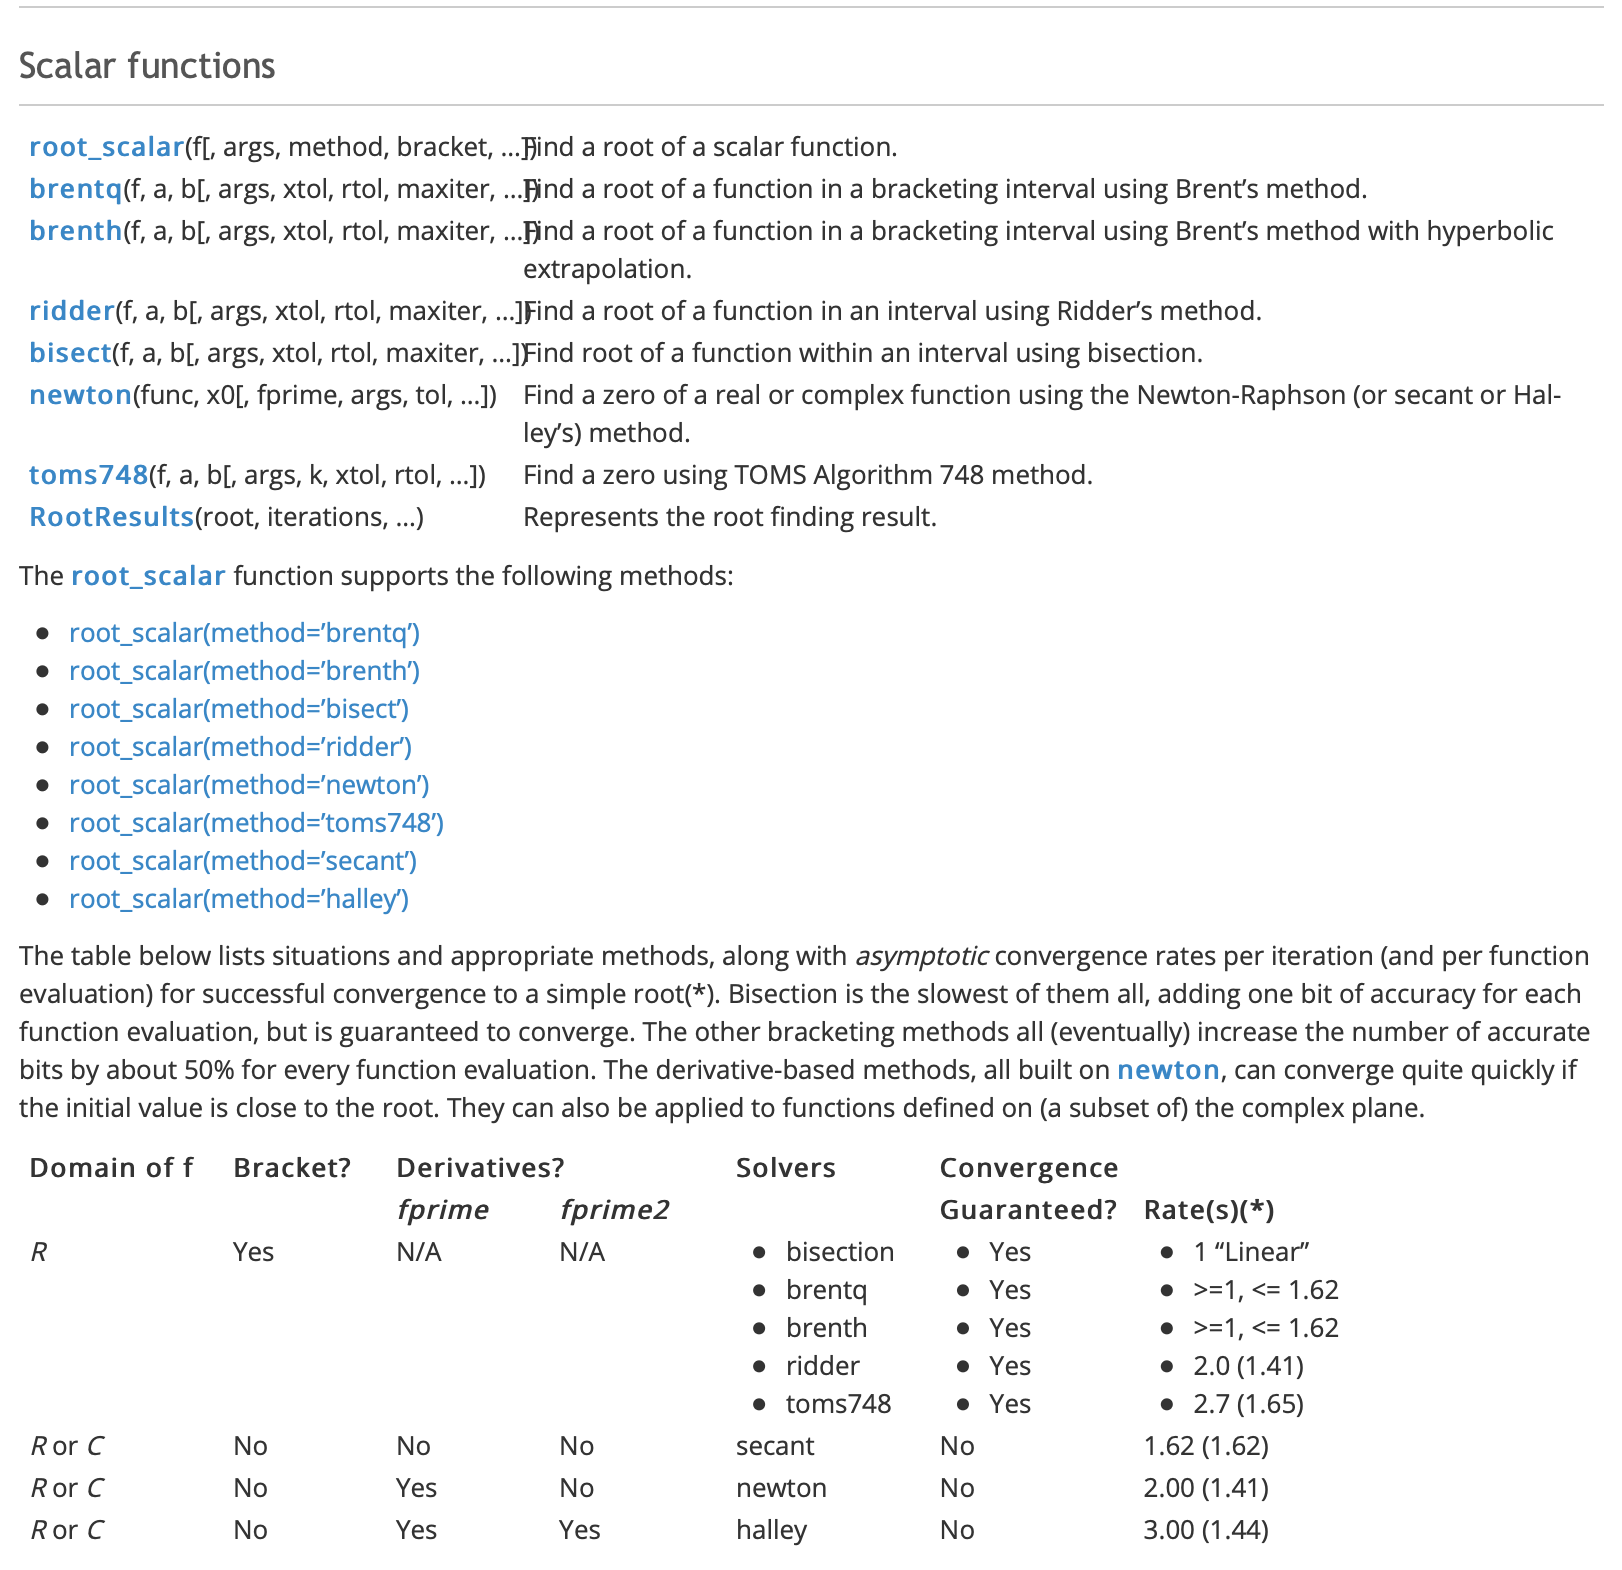
\includegraphics[height=0.9\textheight]{./resources/scipy_roots1.png}
\end{frame}


\section{In higher dimensions...}

\begin{frame}{Multiple Equations}
Solving $f(x) = 0$ for scalars is fine, but we often are interested in $F(\mathbf{x}) = 0$ or $m$ nonlinear equations and $k$ unknowns $\mathbf{x} = (x_1,\ldots, x_K) \in \mathbb{R}^k$.
\begin{itemize}
\item If we have $k>m$ we say the system is \alert{undetermined}
\item If we have $k<m$ we say the system is \alert{overdetermined}
\item I am going to focus on the \alert{square} case of $m$ equations and $m$ unknowns.
\item Think about a system of FOC for prices/quantities/etc.
\end{itemize}
For the most part, the approaches for scalar root finding still apply.
\end{frame}

\begin{frame}{Solution Methods}
\vspace{0.5cm}
General problem $F(\mathbf{x}) = 0$ or $m$ nonlinear equations and $m$ unknowns $\mathbf{x} = (x_1,\ldots, x_m) \in \mathbb{R}^m$.
\begin{eqnarray*}
F_1 (x_1,\ldots, x_m)  &=& 0 \\
F_2 (x_1,\ldots, x_m)  &=& 0\\
&\vdots&\\ 
F_{N-1} (x_1,\ldots, x_m)  &=& 0\\
F_N (x_1,\ldots, x_m)  &=& 0\\
\end{eqnarray*}
\end{frame} 

\begin{frame}{Solution Methods}
Helpful to write $F(\mathbf{x}) = 0 \Leftrightarrow \mathbf{x} - \alpha F(\mathbf{x}) = \mathbf{x}$ which yields the fixed point problem:
\begin{eqnarray*}
G(\mathbf{x}) = \mathbf{x} -\alpha F(\mathbf{x})
\end{eqnarray*}
Fixed point iteration
\begin{eqnarray*}
\mathbf{x^{n+1}} = G(\mathbf{x^n})
\end{eqnarray*}
Nonlinear Richardson iteration or Picard iteration.\\
\vspace{0.5cm}
We need $G$ to be a \alert{contraction mapping} for iterative methods to guarantee a unique solution (often need strong monotonicity as well).
\end{frame} 

\begin{frame}{Gauss Jacobi: Simultaneous Best Reply}
Current iterate: $\mathbf{x^n} = (x_1^n,x_2^n,\ldots,x_{m-1}^n,x_m^n)$.\\
\vspace{0.5cm}
Compute the next iterate $\alert{x^{n+1}}$ by solving one equation in one variable using only values from $\mathbf{x^n}$ : 
\begin{eqnarray*}
F_1 (\alert{x_1^{n+1}},x_2^n \ldots, x_{m-1}^n, x_m^n)  &=& 0 \\
F_2  (x_1^n,\alert{x_2^{n+1}},\ldots,x_{m-1}^n,x_m^n)  &=& 0\\
&\vdots&\\ 
F_{m-1}  (x_1^n,x_2^n,\ldots,\alert{x_{m-1}^{n+1}},x_m^n)  &=& 0\\
F_m  (x_1^n,x_2^n,\ldots,x_{m-1}^n, \alert{x_m^{n+1}})  &=& 0
\end{eqnarray*}
Requires contraction and strong monotonicity.
\end{frame} 

\begin{frame}{Gauss Seidel: Iterated Best Response}
Current iterate: $\mathbf{x^n} = (x_1^n,x_2^n,\ldots,x_{m-1}^n,x_m^n)$.\\
\vspace{0.5cm}
Compute the next iterate $\alert{\mathbf{x^{n+1}}}$ by solving one equation in one variable updating as we go through:
\begin{align*}
F_1 (\alert{x_1^{n+1}},x_2^n \ldots, x_{m-1}^n, x_m^n)  &= 0 \\
F_2  (\alert{x_1^{n+1},x_2^{n+1}},\ldots,x_{m-1}^n,x_m^n)  &= 0\\
&\vdots\\ 
F_{m-1}  (\alert{x_1^{n+1},x_2^{n+1},\ldots,x_{m-1}^{n+1}},x_m^n)  &= 0\\
F_m (\alert{x_1^{n+1},x_2^{n+1},\ldots,x_{m-1}^{n+1}, x_m^{n+1}})  &= 0
\end{align*}
Requires contraction and strong monotonicity.\\
You can speed things up (sometimes) by re-ordering equations.

\end{frame} 

\begin{frame}{Newton-Raphson Method}
\begin{enumerate}
\item Take an initial guess $\mathbf{x^0}$
\item Take a Newton step by solving the following system of linear equations
\begin{eqnarray*}
J_F(\mathbf{x^n}) \mathbf{s^n} = - F(\mathbf{x^n})
\end{eqnarray*}
\item New guess $\mathbf{x^{n+1}} =\mathbf{x^n} + \mathbf{s^n}$ or  $\mathbf{x^{n+1}} =\mathbf{x^n} - J_F^{-1}(\mathbf{x^n})\cdot F(\mathbf{x^n}) $ 
\item Good (Quadratic) Local convergence
\end{enumerate}
\begin{itemize}
\item Requires $J_F$ (Jacobian) to be Lipschitz continuous. 
\item Linearity means we do not need to take the inverse to solve the system\\
 (just QR decomp -- \texttt{backslash} in MATLAB).
\item Non-singularity of $J_F$ is weaker than strong monotonicity (more like PSD).
\end{itemize}
\end{frame} 

\begin{frame}{Why not always do Newton-Raphson?}
\begin{itemize}
\item Often computing or inverting $J_f(\mathbf{x^n})$ is hard.
\item Alternatives focus on simplified ways to compute $J_f(\mathbf{x^n})$ or to update $J_f^{-1}(\mathbf{x^n})$
\begin{itemize}
\item Some techniques similar to \alert{secant method} (Broyden's Method).
\item Also what are known as \alert{quasi-Newton} methods.
\end{itemize}
\item If NR is feasible: start with that!
\end{itemize}
\end{frame} 

\begin{frame}{Broyden's Method}
Idea: approximate the Jacobian $J_f(\mathbf{x^n}) \approx A_n$
\begin{enumerate}
\item Start with $A_0 = \mathbf{I}_m$.
\item Iterate on $\mathbf{x^{n+1}}= \mathbf{x^n} - A_n^{-1} F\left(\mathbf{x^{n}}\right)$
\item Update the Jacobian:
\begin{align*}
A_{n+1}=A_{n}-\frac{F\left(\alert{\mathbf{x^{n+1}}}\right)\left[A_{n}^{-1}  F\left(\mathbf{x^{n}}\right) \right]^{\prime}}{\left[A_{n} F\left(\mathbf{x^{n}}\right) \right]^{\prime}\left[A_{n} F\left(\mathbf{x^{n}}\right) \right]}
\end{align*}
\end{enumerate}
This is meant to be the multivariate version of the \alert{secant method}.
\end{frame} 



\begin{frame}{Broyden-Fletcher-Goldfarb-Shanno (BFGS)}
Same idea, different Jacobian update:
\begin{align*}
d_n &= \mathbf{x^{n+1}} - \mathbf{x^n} \\
g_n &= F(\mathbf{x^{n+1}}) -F(\mathbf{x^n}) \\
A_{n+1}&=A_{n}+\frac{g_{n} g_{n}^{\prime}}{d_{n}^{\prime} g_{n}}-\frac{A_{n} d_{n} d_{n}^{\prime} A_{n}}{d_{n}^{\prime} A_{n} d_{n}}
\end{align*}
Or the Davidson-Fletcher-Powell (DFP) version (operates directly on inverse)
\begin{align*}
A_{n+1}^{-1}=A_{n}^{-1}+\frac{d_{n} d_{n}^{\prime}}{d_{n}^{\prime} g_{n}}-\frac{A_{n}^{-1} g_{n} g_{n}^{\prime} A_{n}^{-1}}{g_{n}^{\prime} A_{n}^{-1} g_{n}}
\end{align*}
Usually BFGS is preferred if you can invert $A$. Both of these preserve \alert{positive definiteness}.
\end{frame} 

\begin{frame}{Derivative Free Methods}
Most methods either calculate the derivative explicitly, or calculate it in course via multiple iterations. There are some exceptions:
\begin{itemize}
\item Powell's method.
\item Nelder-Mead/Simplex.
\end{itemize}
There are some pathological problems for derivative/Jacobian based methods, but mostly these are hard to recommend.
\end{frame} 


\begin{frame}{Least Squares Methods}
Instead of solving $F(\mathbf{x})=0$, we could recast the problem as a least squares minimization problem:
\begin{align*}
\min_{\mathbf{x}} \sum_{m=1}^M \left( F_m(\mathbf{x}) \right) ^2
\end{align*}
\begin{itemize}
\item Ex: \alert{Levenberg-Marquardt}
\item This works surprisingly well (including for overdetermined systems).
\item It takes a convex combination of \alert{gradient steps} and \alert{Newton steps}.
\item We will discus more of this when we talk about \alert{nonlinear optimization}.
\end{itemize}
\end{frame} 


\begin{frame}{\texttt{NumPy}}
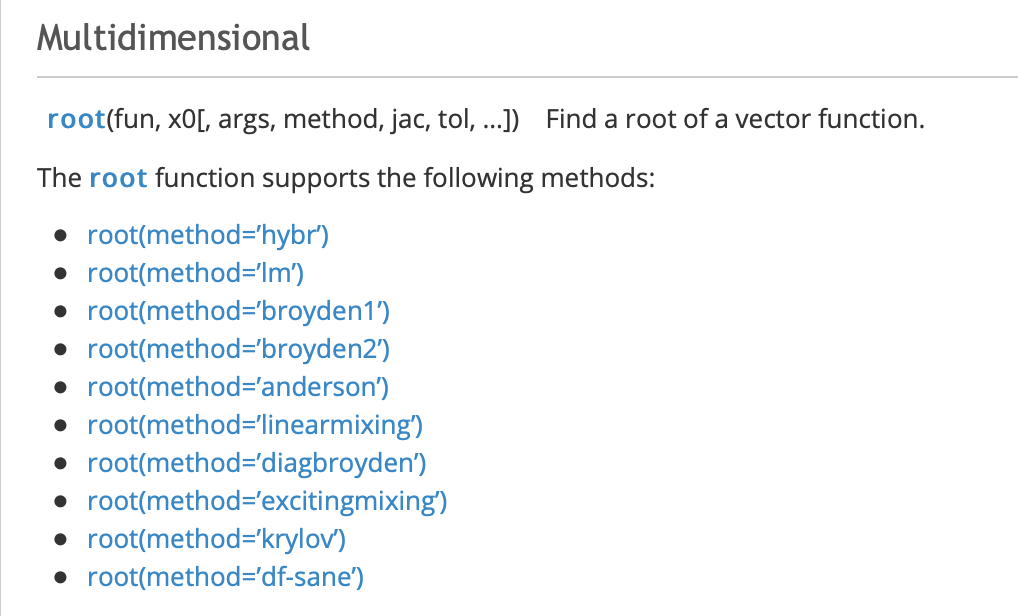
\includegraphics[height=0.9\textheight]{./resources/scipy_roots2.png}
\end{frame}
\section{The end}




\end{document}


